% !TEX TS-program = pdflatex
% !TEX encoding = UTF-8 Unicode

% This file is a template using the "beamer" package to create slides for a talk or presentation
% - Talk at a conference/colloquium.
% - Talk length is about 20min.
% - Style is ornate.

% MODIFIED by Jonathan Kew, 2008-07-06
% The header comments and encoding in this file were modified for inclusion with TeXworks.
% The content is otherwise unchanged from the original distributed with the beamer package.

\documentclass[1pt]{beamer}
\usepackage{media9}
% \usepackage{beamerthemeshadow}
\usepackage[english]{babel}
% or whatever
\usepackage{caption}
\captionsetup[figure]{labelformat=empty}% redefines the caption setup of the figures environment in the beamer class.

\usepackage{units}
\usepackage[utf8]{inputenc}
\usepackage{amsmath}
% \usepackage{fullpage}
\usepackage{amsfonts}
\usepackage{amssymb}
\newcommand{\iu}{{i\mkern1mu}}
\newcommand{\bra}[1]{\langle #1 \vert}
\newcommand{\ket}[1]{\vert#1\rangle}
\newcommand{\avg}[1]{\left\langle#1\right\rangle}
\newcommand{\norm}[1]{\left\Vert #1 \right\Vert}
\newcommand{\braket}[2]{\left\langle #1 \vert#2 \right\rangle}
\newcommand{\obraket}[3]{\left\langle #1 \vert #2 \vert #3 \right \rangle}
\usepackage{times}
\usepackage[T1]{fontenc}
\newcommand{\dd}{\,\mathrm{d}}
\newcommand{\ddd}{\mathrm{d}}
\newcommand{\ii}{\mathrm{i}}
\usepackage{mhchem}
\usepackage{units}
% Copyright 2004 by Till Tantau <tantau@users.sourceforge.net>.
%
% In principle, this file can be redistributed and/or modified under
% the terms of the GNU Public License, version 2.
%
% However, this file is supposed to be a template to be modified
% for your own needs. For this reason, if you use this file as a
% template and not specifically distribute it as part of a another
% package/program, I grant the extra permission to freely copy and
% modify this file as you see fit and even to delete this copyright
% notice. 
\mode<presentation>
{
\usetheme{AnnArbor}
\usecolortheme{crane}
\setbeamertemplate{frametitle}[default][center]
\setbeamertemplate{headline}{}
}

\usepackage{bm}


\title[Anderson localization ] % (optional, use only with long paper titles)
{An introduction to Anderson localization}

%
\includegraphics[width=0.35\textwidth]{logo_fmf_uni-lj_en.pdf}\\[8ex] 

\author[Jan Šuntajs] % (optional, use only with lots of authors)
{Author: Jan Šuntajs \\ 
Mentor: dr. Janez Bonča \\
Comentor: doc. Lev Vidmar}
\centering
\titlegraphic{
\includegraphics[width=4cm]{logo_fmf_uni-lj_en.pdf}
}

% - Give the names in the same order as the appear in the paper.
% - Use the \inst{?} command only if the authors have different
%   affiliation.

%\institute[University of Ljubljana, Faculty of Mathematics and Physics] % (optional, but mostly needed)
%{
%  \inst{1}%
%  Department of Computer Science\\
%  University of Somewhere
%  \and
%  \inst{2}%
%  Department of Theoretical Philosophy\\
%  University of Elsewhere}
% - Use the \inst command only if there are several affiliations.
% - Keep it simple, no one is interested in your street address.

%\date[CFP 2003] % (optional, should be abbreviation of conference name)
%{Conference on Fabulous Presentations, 2003}
% - Either use conference name or its abbreviation.
% - Not really informative to the audience, more for people (including
%   yourself) who are reading the slides online



% If you have a file called "university-logo-filename.xxx", where xxx
% is a graphic format that can be processed by latex or pdflatex,
% resp., then you can add a logo as follows:
%
% \pgfdeclareimage[height=0.8cm]{university-logo}{logo_fmf_uni-lj_en.pdf}
% \logo{\pgfuseimage{university-logo}}

% If you wish to uncover everything in a step-wise fashion, uncomment
% the following command: 

%\beamerdefaultoverlayspecification{<+->}


\begin{document}

\begin{frame}
  \titlepage
\end{frame}

% Structuring a talk is a difficult task and the following structure
% may not be suitable. Here are some rules that apply for this
% solution: 

% - Exactly two or three sections (other than the summary).
% - At *most* three subsections per section.
% - Talk about 30s to 2min per frame. So there should be between about
%   15 and 30 frames, all told.

% - A conference audience is likely to know very little of what you
%   are going to talk about. So *simplify*!
% - In a 20min talk, getting the main ideas across is hard
%   enough. Leave out details, even if it means being less precise than
%   you think necessary.
% - If you omit details that are vital to the proof/implementation,
%   just say so once. Everybody will be happy with that.

% \begin{frame}{Contents}

% \begin{enumerate}
% \item Introduction
% \vspace{10mm}
% \item Theoretical basics
% \vspace{10mm}
% \item Experiments
% \vspace{10mm}
% \item Conclusion
% \end{enumerate}


% \end{frame}


\begin{frame}{What is it about?}
\begin{minipage}[c]{0.5\textwidth}
\begin{itemize}
\item Conduction in \textbf{NON-INTERACTING} systems with \textbf{DISORDER}
\vspace{5mm}
\item Describes the role of \textbf{IMPURITIES}
\vspace{5mm}
\item Completely different than the \textbf{Drude} model:
$$ \sigma \propto l$$
\vspace{5mm}
\end{itemize}
\end{minipage}
\end{frame}

\begin{frame}{What does it predict?}
\begin{minipage}[c]{0.33\textwidth}
\begin{itemize}
\item for some disorder:
$$ \sigma \rightarrow 0$$
\vspace{5mm}
\item put forth by \textbf{P. W. Anderson (1958)}
\vspace{15mm}
\item Nobel prize in \textbf{1977}
% \item \textbf{QPT} at $h_{\perp_c}=J$
\end{itemize}\hfill
\end{minipage}
\begin{minipage}[c]{0.64\textwidth}
\begin{figure}
\centering{
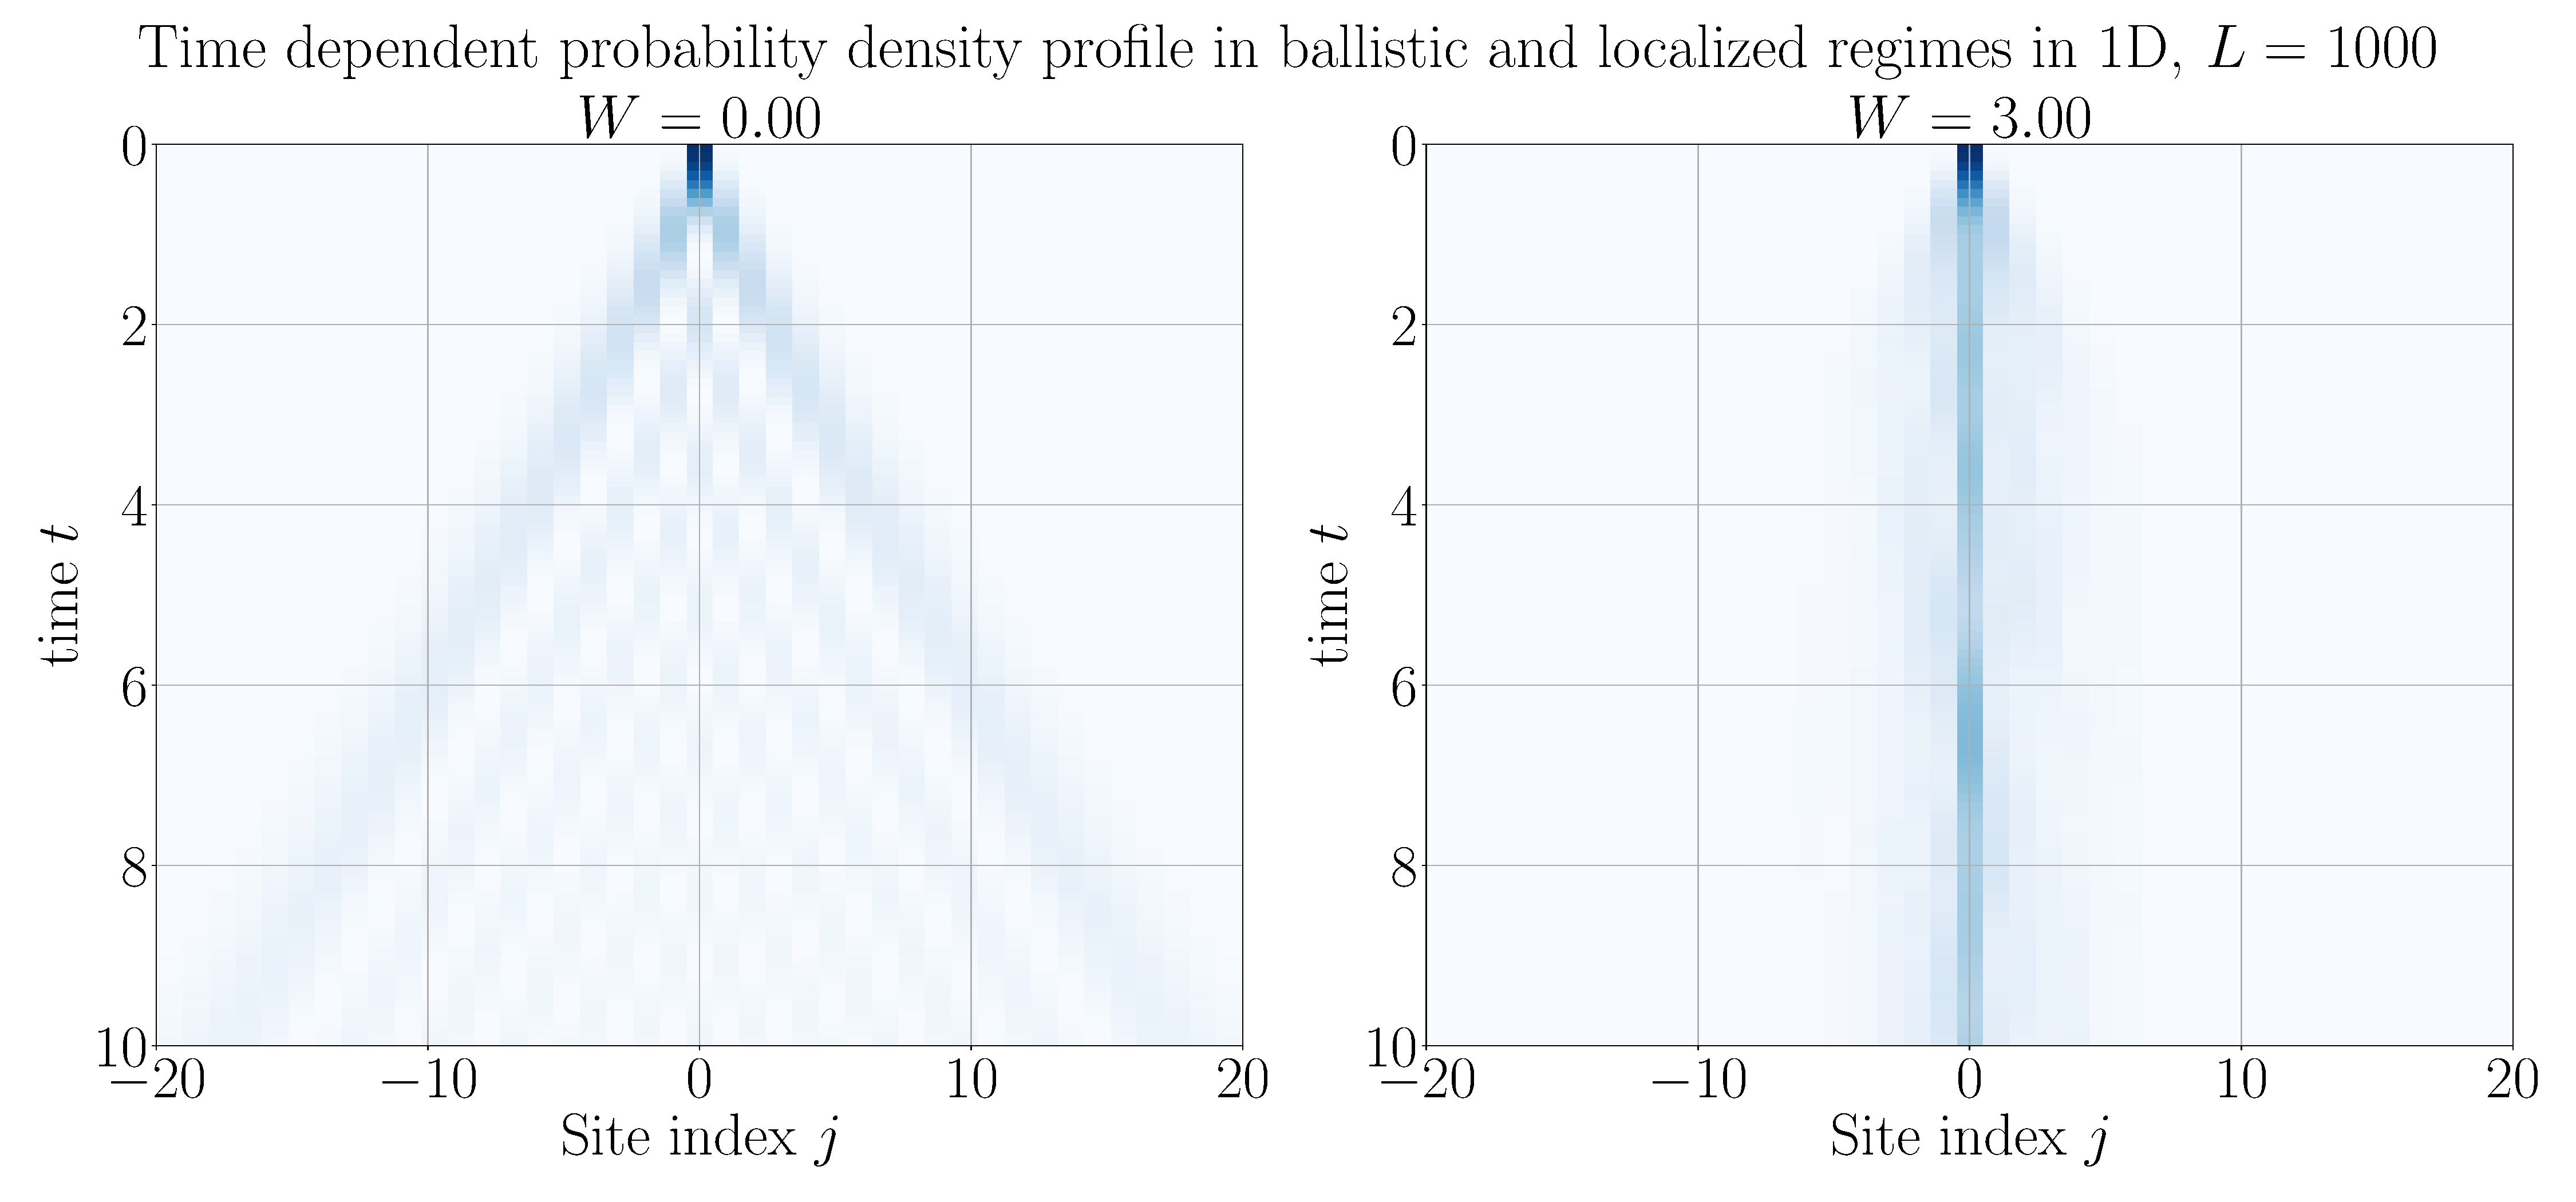
\includegraphics[width=1\textwidth]{1D_Anderson_loc_seminar_D1_shape_1000_light_cone_double.pdf}}
\caption{1D dynamics with no disorder and with strong disorder.}
\end{figure}
\end{minipage}
\end{frame}

\begin{frame}{Why does it (still) matter?}
What began in 1958 ...
\begin{figure}
\centering{

\includegraphics[width=0.9\textwidth]{and_orig_crop.pdf}}
% \caption{}
\end{figure}
... still remains relevant today
\begin{figure}
\centering{

\includegraphics[width=0.8\textwidth]{huse_crop.pdf}}
% \caption{}
\end{figure}
\end{frame}

\begin{frame}{The current ``hot topic''}
\begin{minipage}[c]{0.38\textwidth}
\begin{itemize}
\item \textbf{Many-body localization (MBL)}
\vspace{10mm}
\item includes \textbf{INTERACTIONS}
\vspace{10mm}
\item not our today's topic

\end{itemize}
\end{minipage}
\begin{minipage}[c]{0.6\textwidth}
Published in 2015:
\begin{figure}
\centering{

\includegraphics[width=1\textwidth]{mbl_crop.pdf}}
\caption{672 citations as of April 2018 acc. to Google Scholar.}
\end{figure}
\end{minipage}
\end{frame}

\begin{frame}{Outline}

\begin{enumerate}
\item The basic concepts of the Anderson localization
\vspace{10mm}
\item Models of disorder
\vspace{10mm}
\item Numerical simulations
\vspace{10mm}
\item Conclusion
\end{enumerate}


\end{frame}


% \begin{frame}{The model in a nutshell}
% % \begin{alertblock}{The model Hamiltonian}
% % \begin{equation*}\label{eq:ising_hamiltonian}
% % H_I=-J\sum\limits_i \hat{\sigma}_i^z\hat{\sigma}_{i+1}^z - h_{\perp}\sum\limits_i \hat{\sigma}_{i}^x.
% % \end{equation*}
% % \end{alertblock}{}

% % \begin{minipage}[c]{0.49\textwidth}
% % \begin{figure}
% % \centering{
% % \includegraphics[width=1\textwidth]{Sachdev_phase_diagram.pdf}}
% % \caption{The phase diagram.}
% % \end{figure}
% % \end{minipage}
% % \begin{minipage}[c]{0.4\textwidth}
% % \begin{figure}
% % \centering{
% % \includegraphics[width=1\textwidth]{zigzag_chain.jpg}}
% % \caption{The schematic of cobalt niobate}
% % \end{figure}
% % \end{minipage}\hfill

% \end{frame}

\begin{frame}{The basics}
\begin{minipage}[c]{0.5\textwidth}
\begin{itemize}
\item \textbf{DISORDER} $\rightarrow$ states can localize
\vspace{10mm}
\item A localized state:
$$|\psi(\mathbf{r})| \sim \exp\left(|\mathbf{r} - \mathbf{r}_0 |/\xi \right)$$
\vspace{5mm}
\item explains \textbf{vanishing} transport
\vspace{10mm}
% \item An \textbf{interference} phenomenon.
\end{itemize}
\end{minipage}
\begin{minipage}[c]{0.4\textwidth}
\centering
Localization:
\begin{figure}
\centering{
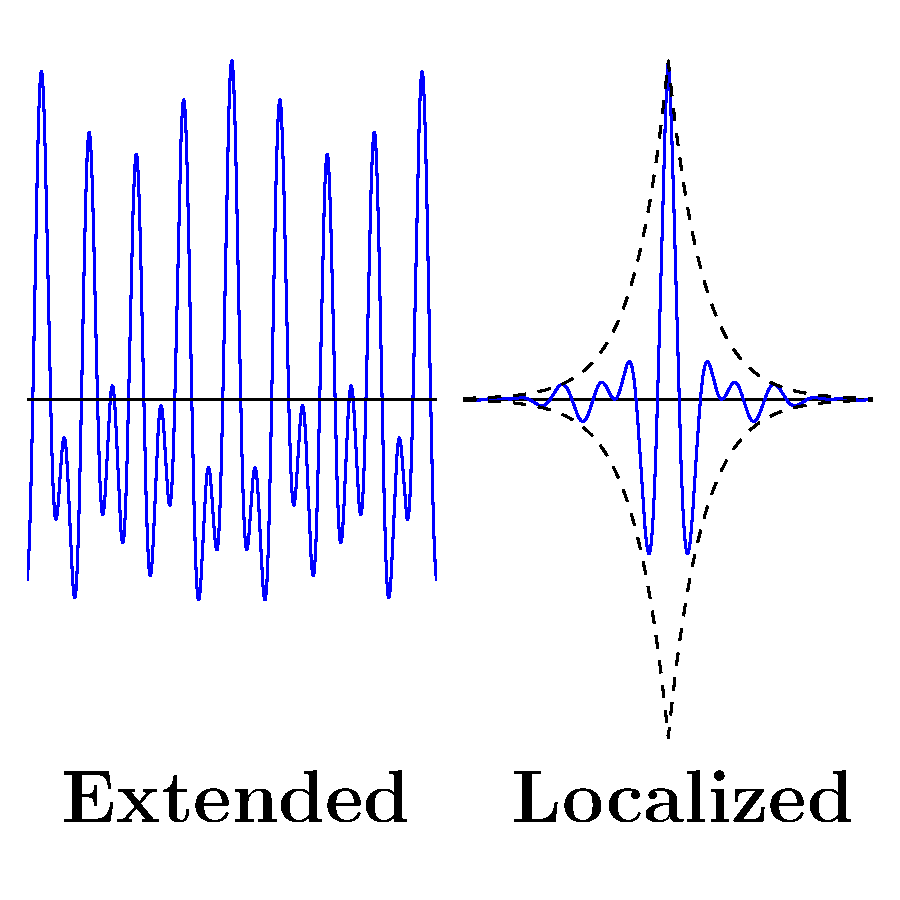
\includegraphics[width=0.88\textwidth]{diff_loc_ext1.pdf}}
\caption{Extended and localized states.}
\end{figure}
\end{minipage}
\end{frame}

\begin{frame}{The important keynotes}
\begin{minipage}[c]{0.5\textwidth}
\begin{itemize}
\item An \textbf{interference} phenomenon
\vspace{8mm}		
\item Strong \textbf{dimensionality} dependence
\vspace{8mm}
\item Energy dependence $\rightarrow$ the \textbf{mobility edge}

% USE THIS LAST BULLET POINT TO INTRODUCE THE NEXT SLIDE
\end{itemize}
\end{minipage}
\end{frame}


\begin{frame}{The enhanced back-scattering}
% REFFER TO NANOPHYSICS HERE !!!! - to those who are attending it
% and to those who did. If they didn't reffer to optics instead
% do not forget RANDOMNESS - PHASES ARE RANDOM, SCATTERING is on
% RANDOM POTENTIALS
\begin{minipage}[c]{0.38\textwidth}
\begin{itemize}
\item calculation of the transition probability $w$
\vspace{5mm}
\item any two paths:
$$w=|A_1 + A_2|^2=w_\mathrm{cl} + w_\mathrm{int}$$
\vspace{5mm}
\item time-reversed paths:
$$w=4|A_1 |^2=2w_\mathrm{cl}$$
% \item \textbf{QPT} at $h_{\perp_c}=J$
\end{itemize}
\end{minipage}\hfill
\begin{minipage}[c]{0.5\textwidth}
\begin{figure}
\centering{
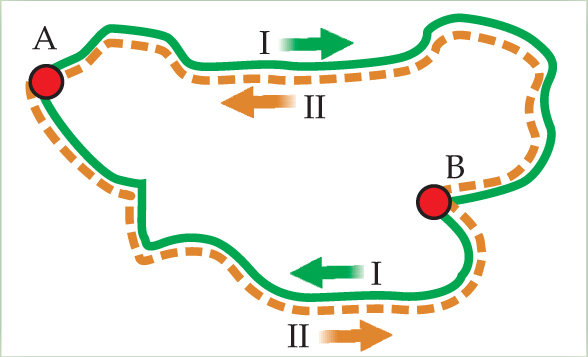
\includegraphics[width=1\textwidth]{interference.jpg}}
\caption{Path from $A$ to $B$ back to $A$ and its time-reverse}
\end{figure}
\end{minipage}
\end{frame}
% BE VERBOSE HERE - MENTION EVERYTHING THAT HAS TO BE SAID, 
% COMMENT THE RESULT; WHAT IT MEANS; WHAT IT CAN DO in 1D and 2D

% \begin{frame}{Theoretical basics}
% % \begin{alertblock}{The model Hamiltonian}
% % \begin{equation*}\label{eq:ising_hamiltonian}
% % H_I=-J\sum\limits_i \hat{\sigma}_i^z\hat{\sigma}_{i+1}^z - h_{\perp}\sum\limits_i \hat{\sigma}_{i}^x.
% % \end{equation*}
% % \end{alertblock}{}

% % \begin{alertblock}{The Pauli matrices}
% % $$
% % \hat{\sigma}_i^z=\begin{pmatrix}
% % 1 & 0 \\ 0 & -1
% % \end{pmatrix}; \hspace{5mm}
% % \hat{\sigma}_i^x=\begin{pmatrix}
% % 0 & 1\\ 1 & 0
% % \end{pmatrix}; \hspace{5mm}
% % \hat{\sigma}_i^y=\begin{pmatrix}
% % 0 & -\iu \\ \iu & 0
% % \end{pmatrix}
% % $$
% % \end{alertblock}{}
% % \begin{alertblock}{The $\hat{\sigma}_i^x$ operator eigenstates}
% % \begin{equation*}
% % \begin{split}
% % \ket{\rightarrow}_i& = \left(\ket{\uparrow}_i + \ket{\downarrow}_i\right)/\sqrt{2}, \\
% % \ket{\leftarrow}_i& = \left(\ket{\uparrow}_i - \ket{\downarrow}_i\right)/\sqrt{2}.
% % \end{split}
% % \end{equation*}
% % \end{alertblock}{}
% \end{frame}

% SAY THAT EBS CAN GIVE AN INTUITIVE EXPLANATION BUT IS 
% INSUFFICIENT IN ACCOUNTING FOR THE COMPLEX DIMENSIONALITY DEPENDENCE
% NOTE THAT THE COMPLETE TREATMENT IS STILL MISSING - WE RESORT TO 
% PHENOMENOLOGICAL THEORIES SUCH AS THE SCALING THEORY
\begin{frame}{The scaling theory }
\begin{minipage}[c]{0.38\textwidth}
\begin{itemize}
\item scaling of the \textbf{conductance} $g$
\vspace{15mm}
\item \textbf{Ohmic} conductor:
$$g=\sigma L^{d-2}$$
\vspace{5mm}
\item \textbf{Localized} regime:
$$g\propto \exp(-L)$$
% \item \textbf{QPT} at $h_{\perp_c}=J$
\end{itemize}
\end{minipage}\hfill
\begin{minipage}[c]{0.6\textwidth}
\begin{figure}
\centering{
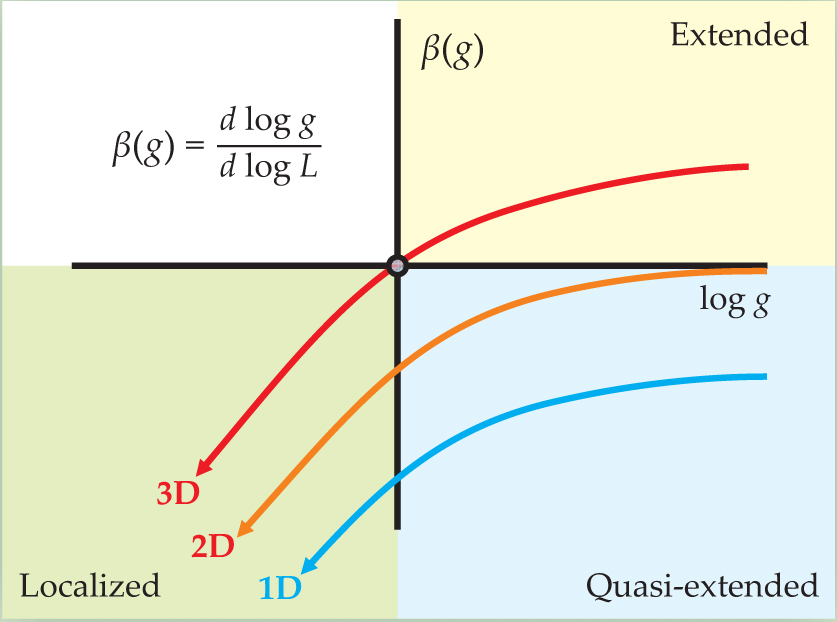
\includegraphics[width=1\textwidth]{beta_diagram.jpg}}
\caption{Transition between ext. and loc. states is only possible in 3D.}
\end{figure}
\end{minipage}
\end{frame}
\begin{frame}{The scaling theory}
\begin{minipage}[c]{0.36\textwidth}
\begin{alertblock}{\centering\textbf{1D, 2D}}
\centering localization for any finite disorder
\end{alertblock}\vspace{0.65cm}
\begin{alertblock}{\centering\textbf{3D}}
\centering localization for some critical disorder
\end{alertblock}\vspace{0.35cm}
\end{minipage}\hfill
\begin{minipage}[c]{0.6\textwidth}
\begin{figure}
\centering{
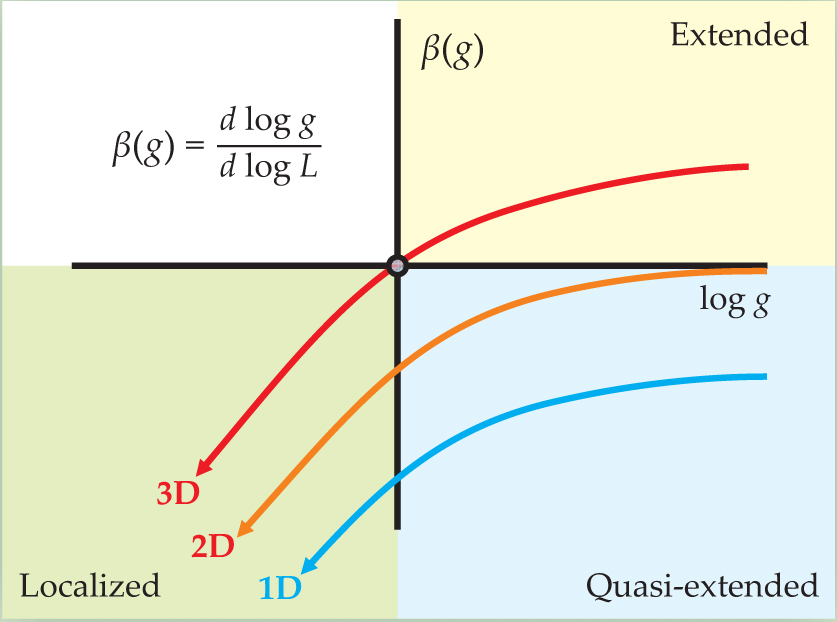
\includegraphics[width=1\textwidth]{beta_diagram.jpg}}
\caption{Transition between ext. and loc. states is only possible in 3D.}
\end{figure}
\end{minipage}
\end{frame}

\begin{frame}{The mobility edge}

\begin{figure}
\centering{
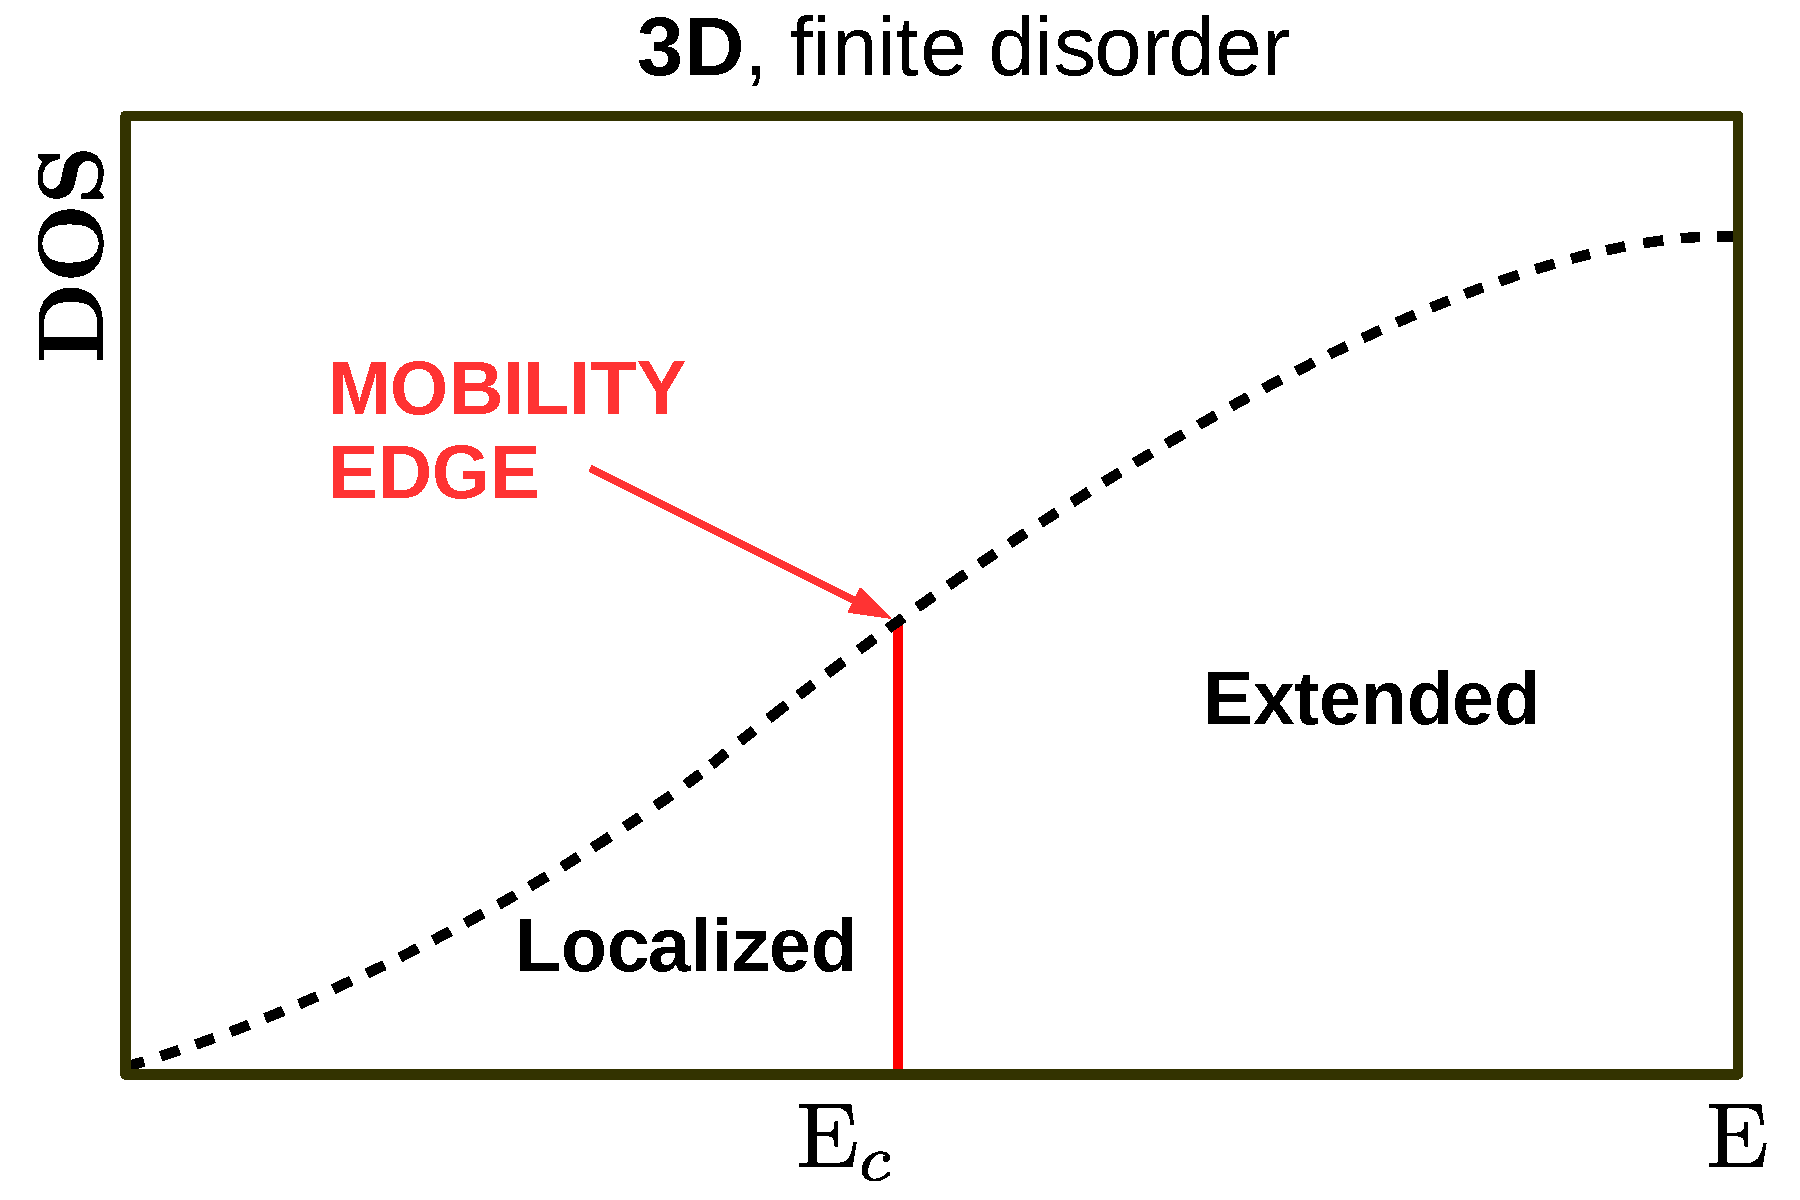
\includegraphics[width=1\textwidth]{mob_edge_schematic.pdf}}
%\caption{Single-excitation dispersion relation}
\end{figure}


\end{frame}

\begin{frame}{The models of disorder}
% \begin{minipage}[c]{0.5\textwidth}
% \begin{equation*}\label{eq:schrodinger}
% -\frac{\hbar^2}{\mu}\frac{\dd^2}{\dd x^2}\Psi(x) + \lambda |x|\Psi(x) = (m-2m_0)\Psi(x).
% \end{equation*}
% \begin{equation*}\label{eq:lastne}
% m_j=2m_0 + z_j \lambda^{2/3} \left(\frac{\hbar^2}{\mu}\right)^{1/3}, \hspace{5mm} j=1,2,3,\dots
% \end{equation*}
% \end{minipage}
% \begin{figure}
% \centering{
% \includegraphics[width=0.65\textwidth]{airy.pdf}}
% \end{figure}
\end{frame}

\begin{frame}{A schematic of the cobalt niobate, $\ce{CoNb_2O6}$}
% \begin{minipage}[c]{0.56\textwidth}
% \begin{itemize}
% \item \large{$\mathbf{J_0}$ ferromagnetic $\sim\unit[18]{K}$} \vspace{5mm}
% \item \large{$\mathbf{J_1}$, $\mathbf{J_2}$ antiferromagnetic}\vspace{5mm}
% \item \large{$\mathbf{J_0} \gg \mathbf{J_1},\ \mathbf{J_2}$}
% \end{itemize}
% \end{minipage}\hfill
% \begin{minipage}[c]{0.43\textwidth}
% \begin{figure}
% \centering{
% \includegraphics[width=1\textwidth]{zigzag_chain.jpg}}
% \end{figure}
% \end{minipage}\\
% \begin{minipage}[c]{0.63\textwidth}
% \begin{figure}
% \centering{
% \includegraphics[width=0.98\textwidth]{spins_structure.pdf}}
% \end{figure}
% \end{minipage}\hfill
% \begin{minipage}[c]{0.35\textwidth}
% \begin{itemize}
% \item $T>\unit[25]{K}$: classical paramagnet
% \item $T<\unit[2.95]{K}$: magnetic order
% \end{itemize}

% \end{minipage}

\end{frame}
\begin{frame}{The neutron scattering experiments}
% \large{The onset of a phase transition at $h_{\perp_c}=\unit[5.5]{T}$}
% \begin{figure}
% \centering{
% \includegraphics[width=1\textwidth]{F2large.jpg}}
% %\caption{Single-excitation dispersion relation}
% \end{figure}
\end{frame}
\begin{frame}{The neutron scattering experiments}
% \large{The effects of the longitudinal field}\\\vspace{10mm}
% \begin{minipage}{0.38\textwidth}
% The continuum splits into discrete states. 
% \begin{figure}
% \centering{
% \includegraphics[width=1\textwidth]{morris_sup_excitations.pdf}}
% %\caption{Single-excitation dispersion relation}
% \end{figure}
% 5 discrete states observed. 
% \end{minipage}\hfill
% \begin{minipage}{0.6\textwidth}
% \begin{figure}
% \centering{
% \includegraphics[width=1\textwidth]{bound_kinks_scatter.pdf}}
% %\caption{The continuum splits into discrete states.}
% \end{figure}
% \end{minipage}
\end{frame}
\begin{frame}{The neutron scattering experiments}
% \begin{minipage}{0.49\textwidth}
% \begin{figure}
% \centering{
% \includegraphics[width=1\textwidth]{bound_kink_peaks.pdf}}
% \caption{Neutron-scattering peaks at the zone center.}
% \end{figure}
% \end{minipage}\hfill
% \begin{minipage}{0.49\textwidth}
% \begin{figure}
% \centering{
% \includegraphics[width=1\textwidth]{bound_kink_matching.pdf}}
% \caption{Matching with the Airy-zeros prediction.}
% \end{figure}
% \end{minipage}
% \large {\textbf{Note}: using a different method, 9 2-kink bound states and a bound state of bound states were measured. }
% \end{frame}

% \begin{frame}{Ideas for further discussion}
% \begin{itemize}
% \item What happens near the \textbf{QCP} where both fields need to be considered?\vspace{5mm}
% \item How to measure all discrete excitations in the kink-confinement model?
% \end{itemize}
\end{frame}





%\begin{frame}{Sources of Images}
%    
%  \begin{thebibliography}{10}
%    
%  \beamertemplatebookbibitems
%  % Start with overview books.
%
%
% 
%    
%  \beamertemplatearticlebibitems
%  % Followed by interesting articles. Keep the list short. 
%
%\bibitem{Tordesillas}
%A. Tordesillas, C. A. H. Steer and D. M. Walker, \emph{Force chain and contact cycle evolution in a dense granular material under shallow penetration}, Nonlin. Processes Geophys. \textbf{21} (2010).
%\bibitem{Muthuswamy}
%M. Muthuswamy, A. Tordesillas,  \emph{How do interparticle contact friction, packing density and degree of polydispersity affect force propagation in particulate assemblies?}, J. Stat. Mech.  \textbf{9} (2006).
%
%\bibitem{Jamming}
%T. Kiwing, P. Lai and H. K. Pak,   \emph{Jamming of Granular Flow in a Two-Dimensional Hopper}, Phys. Rev. Lett.   \textbf{86},1 (2001).
%
%\bibitem{segreggation}
%J. B. Knight, H. M. Jaeger and S. R. Nagel, \emph{Vibration-induced size separation in granular media: The convection connection}, Phys. Rev. Lett. \textbf{70}, 24 (1993)
%
%  \end{thebibliography}
%\end{frame}

\end{document}


